% ==============================================================================
% Artículo científico completo (doble columna) sobre la réplica y extensión
% del conteo de referencias wait-free en arquitecturas híbridas P/E-core.
% Compilación (desde mejoras/paper/):
%   pdflatex paper_wait_free_hibrido_2026.tex && bibtex paper_wait_free_hibrido_2026 && pdflatex paper_wait_free_hibrido_2026.tex && pdflatex paper_wait_free_hibrido_2026.tex
% ==============================================================================
\documentclass[10pt,twocolumn,a4paper]{article}
\usepackage[utf8]{inputenc}
\usepackage[T1]{fontenc}
\usepackage[spanish,es-noshorthands,es-nodecimaldot,es-tabla]{babel}
\spanishplainpercent
\usepackage{geometry}
\geometry{top=1.9cm,bottom=2.0cm,left=1.65cm,right=1.65cm,columnsep=0.6cm}
\usepackage[expansion=false]{microtype}
\usepackage{booktabs,tabularx,array,multirow}
\usepackage{graphicx,float}
\usepackage{amsmath,amssymb}
\usepackage{xcolor}
\usepackage{caption}
\usepackage{fancyhdr}
\usepackage{balance}
\usepackage{cite}
\usepackage{xurl}
\usepackage{tikz}
\usetikzlibrary{arrows.meta,positioning,shapes.geometric,fit,backgrounds}
\usepackage{hyperref}

\definecolor{tinta}{HTML}{1B2430}
\definecolor{gris}{HTML}{5B6573}
\definecolor{acento}{HTML}{C8551F}
\definecolor{azul}{HTML}{1F5FA8}
\definecolor{ok}{HTML}{1B7F3B}
\definecolor{mal}{HTML}{B3261E}
\definecolor{suave}{HTML}{F2F5F9}
\definecolor{suavev}{HTML}{EDF7F0}
\definecolor{suaven}{HTML}{FDF3EE}

\hypersetup{
  colorlinks=true,
  linkcolor=azul,
  urlcolor=azul,
  citecolor=azul,
  pdftitle={Conteo de Referencias Wait-Free en Arquitecturas Hibridas P/E: Replica, Diagnostico Causal y Cuatro Mejoras Incrementales},
  pdfauthor={David Tamo Turpo, Jheremy Manuel Alvarez Astete, Diego Quispe Candelario}
}

\captionsetup{font=footnotesize,labelfont=bf}
\renewcommand{\arraystretch}{1.12}
\graphicspath{{../resultados_v1_v2/figuras/}{../resultados_v3/figuras/}{../resultados_v4/figuras/}{../resultados_i5_10400_comparativa/figuras/}}

\pagestyle{fancy}
\fancyhf{}
\fancyhead[L]{\scriptsize\color{gris}Conteo de Referencias \emph{Wait-Free} en Arquitecturas Híbridas P/E-Core}
\fancyhead[R]{\scriptsize\color{gris}Tamo Turpo, Alvarez Astete \& Quispe Candelario (2026)}
\fancyfoot[C]{\scriptsize\thepage}
\renewcommand{\headrulewidth}{0.4pt}

\begin{document}
\emergencystretch=1.6em

\twocolumn[{%
\begin{@twocolumnfalse}
\begin{center}
  {\small\color{acento}\textbf{ARTÍCULO DE INVESTIGACIÓN Y REPRODUCIBILIDAD EXPERIMENTAL}}\\[4pt]
  {\LARGE\bfseries Conteo de Referencias \emph{Wait-Free} en Arquitecturas Híbridas P/E:\\
  Réplica Causal, Hallazgos de Microarquitectura y Cuatro Mejoras Incrementales}\\[8pt]
  {\normalsize David Tamo Turpo \quad$\cdot$\quad Jheremy Manuel Alvarez Astete \quad$\cdot$\quad Diego Quispe Candelario}\\[3pt]
  {\footnotesize Curso de Computación Paralela y Distribuida --- Noviembre de 2026}\\
  {\footnotesize Réplica base (\texttt{main}): \url{https://github.com/davichiacustico-ux/replica-wait-free-refcount} \quad|\quad Mejoras (\texttt{mejoras-autores}): \url{https://github.com/dtamotu/replica-wait-free-refcount/tree/mejoras-autores}}
\end{center}
\vspace{4pt}

\begin{quote}
\small
\textbf{Resumen---}El conteo de referencias atómico \emph{wait-free} propuesto por de Wolff et al.\ en Euro-Par 2024 elimina las carreras \emph{read-reclaim} sin reclamación diferida, pero su comportamiento sobre procesadores modernos híbridos con núcleos asimétricos (P-cores y E-cores) permanece inexplorado. Presentamos primero una réplica experimental rigurosa del artefacto oficial (14\,158 ejecuciones en un Intel Core Ultra 9 285 de 24 núcleos y contraste en un Core i5-10400) que audita sus 15 afirmaciones y revela fenómenos propios de la microarquitectura híbrida Arrow Lake: una paradoja de coherencia donde los E-cores intra-clúster se comunican $2{,}47\times$ más rápido ($35{,}0$\,ns) que dos P-cores ($86{,}3$\,ns), una bimodalidad causal de latencia de $3{,}4\times$ ($414$ frente a $1\,408$\,ns) según colocación P/E, la inversión del clásico \texttt{\_mm\_pause()} ($-28$ a $-33\,\%$) y una amplificación severa de la inanición en \texttt{compare\_and\_set} (\S 5.1) cuando un escritor en E-core compite contra lectores en P-cores. A partir de este diagnóstico diseñamos, verificamos bajo ASan+UBSan y TSan y evaluamos en ablación (>1\,500 corridas adicionales) cuatro mejoras incrementales sobre \texttt{Autores}: \textbf{\texttt{v1}} (higiene de \texttt{CAS} sin copias ni pre-incremento inútil), \textbf{\texttt{v2}} (bloque de control \emph{in-place} de 32\,B y \texttt{shared\_ptr} de 8\,B), \textbf{\texttt{v3}} (\emph{Elimination-Backoff} linealizable de una sola palabra atómica particionado por clúster L2 y P/E) y \textbf{\texttt{v4}} (\texttt{compare\_and\_set} sin inanición mediante \emph{Fast-Path / Slow-Path} híbrido). En conjunto, \texttt{v2} rompe el techo de $n=10^6$ ($+81\,\%$ a 1\,h, $+39\,\%$ a 24\,h, $-29{,}3\,\%$ de RSS), \texttt{v3} supera a \texttt{Autores}, \texttt{Anderson} y \texttt{Folly} en los \textbf{6 de 6 paneles} de la Figura~5 ($3{,}81\times$ en $n=1, u=50\,\%$, $+65\,\%$ sobre eliminación ciega a topología y escalado positivo de 12 a 24 hilos), y \texttt{v4} logra $4{,}7\times$ mayor rendimiento del escritor y $38\times$ menor latencia \texttt{p99,95} en ataques adversariales E-core manteniendo 0\,\% de sobrecosto en la Figura~6 y 0 bloques diferidos.
\end{quote}
\vspace{6pt}
\end{@twocolumnfalse}
}]

% ==============================================================================
\section{Introducción}
% ==============================================================================

La gestión segura de memoria en estructuras de datos concurrentes sin bloqueos (\emph{lock-free} y \emph{wait-free}~\cite{herlihy1991waitfree}) constituye un pilar crítico de los sistemas paralelos modernos. El conteo de referencias~\cite{collins1960refcount} (\texttt{std::shared\_ptr} en C++~\cite{sutter2014atomic}) ofrece reclamación inmediata —evitando las pausas de cola y la acumulación de memoria propias de los esquemas basados en épocas o punteros de peligro~\cite{michael2004hazard,kim2024epochs}—, pero al compartirse mediante una celda atómica sufre la carrera \emph{read-reclaim}: un hilo lector puede leer la dirección de un objeto justo antes de que un escritor lo reemplace y libere, provocando errores \emph{use-after-free}~\cite{chen2023uaf}.

En Euro-Par 2024, de Wolff, Anderson, Keller y Seletskiy~\cite{dewolff2024waitfree} propusieron una solución \emph{wait-free} para \texttt{load()} y \texttt{store()} sobre punteros compartidos atómicos combinando conteo ponderado~\cite{bevan1987weighted,watson1987weighted} con un protocolo acotado de recarga de peso en $O(P)$ pasos (donde $P$ es el número de hilos), logrando cero sobrecoste espacial diferido frente a \texttt{Anderson} (CDRC~\cite{anderson2021cdrc,anderson2022turning}) y evitando las instrucciones \texttt{cmpxchg16b} en bucle de \texttt{Williams}~\cite{williams2012concurrency} y \texttt{Folly}~\cite{folly2024}. Sin embargo, su evaluación experimental se restringió a servidores homogéneos Xeon (72 núcleos/144 hilos DDR4 y 28 núcleos/56 hilos DDR5), dejando abiertas tres preguntas fundamentales:
\begin{enumerate}
  \item \textbf{¿Qué ocurre en procesadores híbridos modernos (P-cores + E-cores)?} Las arquitecturas heterogéneas como Intel Arrow Lake introducen latencias de coherencia fuertemente asimétricas entre clústeres L2 y diferencias de velocidad entre núcleos que pueden invalidar supuestos clásicos de sincronización~\cite{schone2024alderlake,liu2022libasl}.
  \item \textbf{¿Qué parte de las brechas medidas proviene del algoritmo y cuál de detalles de implementación?} Como advierten Mytkowicz et al.~\cite{mytkowicz2009wrongdata}, decisiones invisibles de asignación, banderas de compilación o paso por valor pueden invertir el orden relativo entre sistemas.
  \item \textbf{¿Pueden resolverse simultáneamente la contención extrema, el techo de ancho de banda y la limitación teórica del \S 5.1 sin sacrificar la liberación inmediata?}
\end{enumerate}

\textbf{Contribuciones principales.} Partiendo de nuestra réplica cerrada del artefacto oficial de Zenodo~\cite{dewolff2024artifact,replica2026ultra9} (14\,158 ejecuciones), este trabajo aporta:
\begin{itemize}
  \item \textbf{Caracterización causal de la arquitectura híbrida Arrow Lake} sobre primitivas atómicas (paradoja L2 intra-clúster vs.\ P-cores, bimodalidad P/E de $3{,}4\times$, efecto negativo de \texttt{\_mm\_pause()}, inversión frente a un Core i5-10400 homogéneo y asimetría de inanición P-contra-E).
  \item \textbf{Auditoría empírica de reproducibilidad} con tres hallazgos metodológicos propios: el candado oculto en el binario de latencia de Williams sin \texttt{-mcx16}, el doble efecto de \texttt{alignas(128)} y la detección del coste de doble asignación del C++ oficial.
  \item \textbf{Cuatro mejoras incrementales verificadas (\texttt{Autores-v1} a \texttt{Autores-v4})}~\cite{mejoras2026autores}, cada una sustentada en literatura clásica y reciente, validada con ASan+UBSan, TSan y \texttt{bench\_basura} (0 errores, 0 \emph{data races}, 0 bloques diferidos) y medida en ablación estricta frente a controles transparentes.
\end{itemize}

% ==============================================================================
\section{Metodología y Pipeline Experimental}
% ==============================================================================

La Figura~\ref{fig:pipeline} resume el \emph{pipeline} científico de extremo a extremo del proyecto, diseñado siguiendo las directrices de Hoefler y Belli~\cite{hoefler2015benchmarking}.

\begin{figure*}[t]
\centering
\resizebox{\linewidth}{!}{%
\begin{tikzpicture}[
  node distance=0.45cm and 0.55cm,
  box/.style={rectangle, rounded corners=4pt, draw=#1, fill=#1!8, line width=0.8pt,
              align=center, font=\scriptsize, inner sep=5pt, minimum height=1.15cm},
  arr/.style={-{Stealth[length=2.2mm]}, thick, color=tinta}
]
  \node[box=azul, text width=2.85cm] (p1) {\textbf{1. Réplica Base}\\\texttt{main} (\texttt{17f1e45})\\14\,158 corridas\\Ultra 9 + i5-10400\\Artefacto Zenodo};
  \node[box=acento, right=of p1, text width=3.05cm] (p2) {\textbf{2. Diagnóstico Causal}\\4 cuellos de botella:\\6 RMW en \texttt{CAS},\\doble \texttt{new} DDR5,\\L2/P-E, inanición \S 5.1};
  \node[box=ok, right=of p2, text width=3.3cm] (p3) {\textbf{3. Escalera \texttt{v1}$\to$\texttt{v4}}\\\texttt{v1}: \texttt{CAS} ref+precheck\\\texttt{v2}: \emph{in-place} 32\,B + 8\,B\\\texttt{v3}: Elim.\ L2 + P/E\\\texttt{v4}: \texttt{CAS} Fast/Slow};
  \node[box=azul, right=of p3, text width=2.9cm] (p4) {\textbf{4. Verificación}\\ASan + UBSan\\TSan (\texttt{setarch -R})\\Cota $P=32,C=64$\\\texttt{bench\_basura} (0 dif.)};
  \node[box=tinta, right=of p4, text width=3.0cm] (p5) {\textbf{5. Ablación Final}\\885 rend.\ + 390 Fig.~6\\+ 50 adv.\ 23L+1E\\Controles: \texttt{v1p/v2p},\\\texttt{v3a/v3g}, \texttt{And-v3}};

  \draw[arr] (p1) -- (p2);
  \draw[arr] (p2) -- (p3);
  \draw[arr] (p3) -- (p4);
  \draw[arr] (p4) -- (p5);

  % Feedback arrow for reentrancy bug found in v4
  \draw[arr, dashed, color=mal] (p5.south) -- ++(0,-0.32) -| node[pos=0.25, below, font=\tiny\color{mal}]{Fix reentrancia \texttt{drain\_local()} (\texttt{v4}) y ablación negativa \texttt{\_mm\_pause()} (\texttt{v1p/v2p})} (p3.south);
\end{tikzpicture}%
}
\caption{Pipeline metodológico completo del estudio: desde la réplica cerrada del paquete de Zenodo hasta la ingeniería, verificación con sanitizers y ablación controlada de \texttt{Autores-v1} a \texttt{Autores-v4}.}
\label{fig:pipeline}
\end{figure*}

\textbf{Plataformas de medición.} La máquina principal es un \textbf{Intel Core Ultra 9 285} (Arrow Lake, 24 núcleos físicos sin SMT: 8 P-cores \texttt{cpu0..7} con L2 privada y 16 E-cores \texttt{cpu8..23} agrupados en 4 clústeres L2 de 4 núcleos, 36\,MB L3 compartida, 1$\times$32\,GB DDR5-5600, Linux x86-64, \texttt{g++-12} 12.4 con \texttt{-O3 -mcx16}). Como control homogéneo en la réplica se empleó un \textbf{Intel Core i5-10400} (6 núcleos físicos / 12 hilos SMT, DDR4).

\textbf{Disciplina de medición.} Cada punto se ejecuta en un proceso independiente en orden aleatorizado por ronda sobre máquina libre (una sola prueba a la vez, monitorizando temperaturas en 72--85\,°C), usando \texttt{jemalloc} vía \texttt{LD\_PRELOAD} y \texttt{numactl -i all} en rendimiento (\texttt{bench\_stack}, mediana de 3 rondas $\times$ 2\,s; validado frente a la receta $10\,\text{s}\times 7$ del paper dentro de $-1{,}7\,\%$ a $+4{,}3\,\%$ en \texttt{Autores}~\cite{replica2026ultra9}). Para latencia (\texttt{bench\_atomic\_shared\_ptrs}) y el banco adversarial (\texttt{bench\_adversarial\_v4}) fijamos la afinidad de hilos mediante nuestro \emph{shim} \texttt{fijar\_hilos.so}. La memoria diferida se cuantifica con \texttt{bench\_basura} (interceptando \texttt{operator new/delete}) y el pico residente mediante \texttt{ru\_maxrss}.

% ==============================================================================
\section{Hallazgos de la Réplica y de la Arquitectura Híbrida Arrow Lake}
% ==============================================================================

Al contrastar las 15 afirmaciones experimentales de Euro-Par 2024 en nuestra réplica~\cite{replica2026ultra9}, \textbf{9 se reproducen} (ausencia de \emph{use-after-free}, cota $O(P)$ holgada con máximo 8 reintentos frente a $P=32$, 0 bloques diferidos frente a $\approx 29\,000$ en Anderson y menor latencia de \texttt{load}), \textbf{2 se cumplen en parte}, \textbf{3 no se reproducen} (gran ventaja sobre Folly ya a 1 hilo y liderazgo en $n=10^6$) y \textbf{1 no se confirma}. Más reveladores aún fueron los hallazgos sobre la interacción entre primitivas atómicas y la topología híbrida Arrow Lake (Figura~\ref{fig:arrowlake}).

\begin{figure*}[t]
\centering
\resizebox{\linewidth}{!}{%
\begin{tikzpicture}[
  pcore/.style={rectangle, rounded corners=3pt, draw=azul, fill=azul!12, font=\tiny\bfseries, minimum width=1.15cm, minimum height=0.58cm, align=center},
  ecore/.style={rectangle, rounded corners=2pt, draw=ok, fill=ok!12, font=\tiny, minimum width=0.56cm, minimum height=0.45cm, align=center},
  cluster/.style={rectangle, rounded corners=4pt, draw=ok!80!black, fill=suavev, inner sep=4pt},
  bus/.style={rectangle, rounded corners=3pt, draw=tinta, fill=suave, font=\scriptsize\bfseries, minimum width=15.6cm, minimum height=0.52cm, align=center},
  elim/.style={rectangle, rounded corners=2pt, draw=acento, fill=suaven, font=\tiny\bfseries, inner sep=2.5pt}
]
  % 8 P-cores on top
  \foreach \i in {0,...,7} {
    \node[pcore] (p\i) at (\i*1.95, 2.35) {P\i\\{\tiny L2 priv.}};
  }
  \node[elim] at (2.92, 3.05) {Dominio P0 (\texttt{v3})};
  \node[elim] at (10.72, 3.05) {Dominio P1 (\texttt{v3})};

  % Shared L3 Ring
  \node[bus] (l3) at (6.82, 1.35) {Anillo / Caché L3 Compartida (36\,MB) \quad$\longleftrightarrow$\quad Controladora 1$\times$32\,GB DDR5-5600 (canal único)};

  % 4 E-core clusters on bottom
  \foreach \c/\lbl/\a/\b in {0/E0 (8--11)/8/11, 1/E1 (12--15)/12/15, 2/E2 (16--19)/16/19, 3/E3 (20--23)/20/23} {
    \begin{scope}[shift={(\c*4.0 + 0.12, -0.35)}]
      \node[cluster, minimum width=3.45cm, minimum height=1.22cm] (ec\c) at (0.85, 0) {};
      \node[font=\tiny\bfseries\color{ok!80!black}] at (0.85, 0.42) {\lbl\ $\cdot$ L2 \textbf{35\,ns}};
      \node[ecore] at (-0.42, 0.0) {E};
      \node[ecore] at (0.42, 0.0) {E};
      \node[ecore] at (1.26, 0.0) {E};
      \node[ecore] at (2.10, 0.0) {E};
      \node[elim] at (0.85, -0.45) {Ranura Elim.\ L2 (\texttt{v3})};
    \end{scope}
  }

  % Latency annotations
  \draw[{Stealth[length=1.8mm]}-{Stealth[length=1.8mm]}, color=mal, thick] (p0.south) -- (p0.south |- l3.north);
  \draw[{Stealth[length=1.8mm]}-{Stealth[length=1.8mm]}, color=mal, thick] (p7.south) -- (p7.south |- l3.north);
  \node[font=\tiny\bfseries\color{mal}, fill=white, inner sep=1.5pt] at (3.85, 1.84) {P$\leftrightarrow$P: \textbf{86{,}3\,ns} ($2{,}47\times$) \quad|\quad P$\leftrightarrow$E: \textbf{67{,}4\,ns} ($1{,}93\times$)};

  \draw[{Stealth[length=1.8mm]}-{Stealth[length=1.8mm]}, color=ok!80!black, thick] (ec0.north) -- (ec0.north |- l3.south);
  \draw[{Stealth[length=1.8mm]}-{Stealth[length=1.8mm]}, color=ok!80!black, thick] (ec1.north) -- (ec1.north |- l3.south);
  \draw[{Stealth[length=1.8mm]}-{Stealth[length=1.8mm]}, color=ok!80!black, thick] (ec2.north) -- (ec2.north |- l3.south);
  \draw[{Stealth[length=1.8mm]}-{Stealth[length=1.8mm]}, color=ok!80!black, thick] (ec3.north) -- (ec3.north |- l3.south);
  \node[font=\tiny\bfseries\color{ok!80!black}, fill=white, inner sep=1.5pt] at (7.0, 0.68) {E$\leftrightarrow$E mismo clúster: \textbf{35{,}0\,ns} ($1{,}00\times$) \quad|\quad E$\leftrightarrow$E distinto clúster: \textbf{47{,}4\,ns} ($1{,}35\times$)};
\end{tikzpicture}%
}
\caption{Topología medida del Intel Core Ultra 9 285 (Arrow Lake) y su explotación algorítmica: los 4 clústeres E comparten L2 con coherencia $2{,}47\times$ más rápida que dos P-cores, permitiendo el intercambio local de \texttt{Autores-v3}; la asimetría inversa P-vs-E motiva la protección anti-inanición de \texttt{Autores-v4}.}
\label{fig:arrowlake}
\end{figure*}

\subsection{Cinco hallazgos reveladores de la arquitectura híbrida}

\textbf{1. Paradoja de coherencia L2 (E-cores locales $2{,}47\times$ más rápidos que P-cores).} Nuestras mediciones núcleo a núcleo (Cuadro~\ref{tab:c2c}) muestran que dos E-cores del mismo clúster L2 intercambian una línea de caché en \textbf{35{,}0\,ns}, frente a \textbf{47{,}4\,ns} entre clústeres E distintos, \textbf{67{,}4\,ns} entre P y E, y \textbf{86{,}3\,ns} entre dos P-cores. Por ello, al dispersar solo 2--4 hilos fuera de un clúster L2 (\texttt{E-compacto} $\to$ \texttt{E-disperso}), \texttt{Autores} pierde \textbf{$-43\,\%$ a $-54\,\%$} y \texttt{Williams} (\texttt{cmpxchg16b}) colapsa hasta \textbf{$-99\,\%$}. Esta misma penalización inter-clúster explica la \textbf{inversión frente al Core i5-10400}: bajo alta contención a 12 hilos, el modesto procesador homogéneo de 6 núcleos supera al Core Ultra 9 285 (\textbf{39{,}13} frente a \textbf{21{,}79\,Mop/s})~\cite{replica2026ultra9}.

\begin{table}[H]
\centering
\caption{Latencia de coherencia núcleo a núcleo medida en el Core Ultra 9 285 y penalización al cruzar clústeres L2 (2 hilos).}
\label{tab:c2c}
\footnotesize
\begin{tabular}{@{}l r r@{}}
\toprule
\textbf{Clase de comunicación} & \textbf{Mediana (ns)} & \textbf{Relación} \\
\midrule
E $\leftrightarrow$ E (mismo clúster L2) & \textbf{35{,}0} & 1{,}00$\times$ \\
E $\leftrightarrow$ E (clústeres distintos) & 47{,}4 & 1{,}35$\times$ \\
P $\leftrightarrow$ E (anillo L3) & 67{,}4 & 1{,}93$\times$ \\
P $\leftrightarrow$ P (anillo L3) & \textbf{86{,}3} & \textbf{2{,}47$\times$} \\
\bottomrule
\end{tabular}
\end{table}

\textbf{2. Bimodalidad causal de latencia P-core vs.\ E-core.} En la réplica sin afinidad, la latencia \texttt{load} a 24 hilos fluctuaba erráticamente entre $\approx 414$\,ns y $\approx 1\,450$\,ns (razón máx/mín $5{,}75\times$). Al fijar el hilo medido en un P-core (\texttt{todos24-P}), la dispersión entre 5 rondas colapsa a \textbf{$1{,}04\times$} ($405\text{--}421$\,ns); al fijarlo en un E-core (\texttt{todos24-E}), la mediana salta a \textbf{$1\,277\text{--}1\,408$\,ns} ($3{,}4\times$ mayor). En CPUs híbridas, medir latencias sin fijación de afinidad mezcla dos distribuciones físicas distintas~\cite{schone2024alderlake}.

\textbf{3. Inversión del clásico \texttt{\_mm\_pause()} en Arrow Lake.} Contrario a la recomendación clásica de Mellor-Crummey y Scott~\cite{mellorcrummey1991mcs}, nuestra ablación demuestra que insertar \texttt{\_mm\_pause()} en el bucle \texttt{CAS} degrada el rendimiento entre \textbf{$-28\,\%$ y $-33\,\%$} bajo contención ($1{,}63 \to 1{,}10$\,Mop/s en $n=1, u=50\,\%$), porque la latencia moderna de \texttt{PAUSE} ($\sim 140$ ciclos) excede la coherencia intra-clúster L2.

\textbf{4. Asimetría extrema de inanición (P-cores contra E-core).} Cuando un escritor \texttt{compare\_and\_set} corre en un E-core y 23 lectores —incluidos los 8 P-cores— bombardean \texttt{load()}, la asimetría de frecuencia y despacho amplifica drásticamente el problema del \S 5.1: \texttt{Folly} cae a $0{,}3$\,Kops/s y \texttt{Autores-v2} pierde $16\times$ frente a su rendimiento en P-core ($717 \to 44{,}4$\,Kops/s).

\textbf{5. Otros hallazgos metodológicos de la réplica.} Documentamos además un candado oculto en el binario de latencia de Williams al omitirse \texttt{-mcx16}, el doble efecto de \texttt{alignas(128)} ($+3{,}40\times$ en $n=10$ al eliminar \emph{false sharing}, pero $-24\text{--}27\,\%$ en $n=10^6$ al desbordar los 36\,MB de L3) y el coste oculto de liberación diferida por lotes en Anderson ($25\,524\text{--}29\,094$ bloques retenidos y picos \texttt{p99,95} de $7\,731\text{--}7\,770$\,ns en \texttt{store-del} a $p=1$~\cite{kim2024epochs}, frente a $32$\,ns en \texttt{Autores}).

% ==============================================================================
\section{Diseño de las Cuatro Mejoras Incrementales (\texttt{v1} a \texttt{v4})}
% ==============================================================================

Cada mejora ataca un cuello de botella medido sin comprometer el progreso \emph{wait-free} de \texttt{load}/\texttt{store} ni la liberación inmediata.

\subsection{\texttt{Autores-v1}: Higiene de \texttt{CAS} sin copias ni RMW espurias}
La inspección del C++ oficial (\texttt{atomic\_shared\_ptr.h}, L311--348) reveló que \texttt{compare\_exchange\_weak} pasaba \texttt{expected} y \texttt{new\_ptr} \textbf{por valor} a \texttt{compare\_and\_set} (a diferencia de su propio Rust \texttt{arc.rs} y de \texttt{parlay}~\cite{anderson2022turning}), ejecutando hasta \textbf{6 RMW atómicas inútiles} por fallo e incrementando \texttt{new\_cb} antes de comprobar si el puntero actual coincidía con \texttt{expected}. Inspirados en el principio \emph{test-and-test-and-set}~\cite{mellorcrummey1991mcs}, \texttt{Autores-v1} añade sobrecargas por \texttt{const\&}/\texttt{\&\&}, un pre-chequeo de lectura previo a tocar \texttt{new\_cb}, \texttt{rc\_increment\_relaxed} para referencias ya poseídas y el parámetro de ablación \texttt{UsePause} (\texttt{v1} vs.\ \texttt{v1p}).

\subsection{\texttt{Autores-v2}: Bloque de control \emph{in-place} de 32\,B y \texttt{shared\_ptr} de 8\,B}
Mientras el propio paper asume el contador contiguo al objeto (\S 2.1, Fig.~1a~\cite{dewolff2024waitfree}) y los cuatro rivales implementan asignación única~\cite{dimov2007n2351,anderson2022turning}, solo el C++ oficial realizaba dos \texttt{new}/\texttt{delete} separados con clase base virtual y un \texttt{shared\_ptr} de 16\,B. \texttt{Autores-v2} (Figura~\ref{fig:layout}) incrusta \texttt{T} dentro de \texttt{ptr\_control\_block<T>} sin \emph{vtable} (unión híbrida con soporte de punteros externos), compacta \texttt{shared\_ptr<T>} a \textbf{8\,B} (reduciendo cada nodo de la pila + bloque de control a una única reserva de 32\,B) y elimina la indirección adicional \texttt{control\_block->ptr} en \texttt{load()}.

\begin{figure}[H]
\centering
\begin{tikzpicture}[
  mem/.style={rectangle, draw=#1, fill=#1!10, font=\tiny, minimum height=0.52cm, align=center, inner sep=3pt},
  arr/.style={-{Stealth[length=1.8mm]}, semithick, color=tinta}
]
  % Original
  \node[font=\scriptsize\bfseries\color{mal}, anchor=west] at (0, 1.55) {Autores original (2 asignaciones, doble indirección):};
  \node[mem=mal, minimum width=1.65cm] (sp0) at (0.85, 0.95) {\texttt{shared\_ptr}\\(16\,B: \texttt{ptr, cb})};
  \node[mem=gris, minimum width=2.05cm] (cb0) at (3.35, 0.95) {\texttt{control\_block}\\(\texttt{vptr}, \texttt{rc}, \texttt{ptr})};
  \node[mem=gris, minimum width=1.75cm] (nd0) at (5.95, 0.95) {\texttt{Node}\\(\texttt{t}, \texttt{next}:16\,B)};
  \draw[arr] (sp0.east) -- (cb0.west);
  \draw[arr] (cb0.east) -- (nd0.west);

  % v2
  \node[font=\scriptsize\bfseries\color{ok}, anchor=west] at (0, 0.25) {\texttt{Autores-v2} (1 asignación \emph{in-place} de 32\,B, 0 indirección extra):};
  \node[mem=ok, minimum width=1.65cm] (sp2) at (0.85, -0.35) {\texttt{shared\_ptr}\\(\textbf{8\,B}: solo \texttt{cb})};
  \node[mem=ok, minimum width=4.1cm] (cb2) at (4.45, -0.35) {\texttt{ptr\_control\_block<Node>} (32\,B, sin \emph{vtable})\\{\texttt{rc}:8\,B \ |\ \texttt{inplace}:1\,B \ |\ \texttt{Node(t, next:8\,B)}}};
  \draw[arr] (sp2.east) -- (cb2.west);
\end{tikzpicture}
\caption{Rediseño de memoria en \texttt{Autores-v2}: elimina el doble \texttt{new}/\texttt{delete}, la \emph{vtable} y el salto serial en caché/DDR5.}
\label{fig:layout}
\end{figure}

\subsection{\texttt{Autores-v3}: \emph{Elimination-Backoff} consciente de clústeres L2 y P/E}
Para resolver la contención extrema de una sola pila ($n=1$) explotando la paradoja L2 de Arrow Lake (35\,ns intra-clúster), \texttt{Autores-v3} combina tres ideas de la literatura~\cite{hendler2004elimination,liu2022libasl,ouyang2022coreaware}:
\begin{enumerate}
  \item \textbf{Detector automático de topología (\texttt{pe\_topology.h}):} lee una vez \path{/sys/devices/system/cpu/cpu*/cache/index2/shared_cpu_list} para asignar los 4 clústeres E a 4 dominios locales y los 8 P-cores a 2 dominios P (6 dominios en total).
  \item \textbf{Intercambiador de una palabra atómica (\texttt{elimination\_table\_v3.h}):} cada ranura (\texttt{alignas(128)}) es un único \texttt{std::atomic<uint64\_t>} que empaqueta valor (32\,b) + versión monotónica (30\,b, libre de ABA) + estado (\texttt{EMPTY}, \texttt{PUSH\_WAIT}, \texttt{POP\_WAIT}, \texttt{POP\_GOT}). La tabla se asigna perezosamente aprovechando el relleno libre de \texttt{alignas(128)} en \texttt{atomic\_stack}, garantizando \textbf{0 bytes extra en $n=10^6$}. Las ventanas de giro son diferenciadas sin \texttt{\_mm\_pause()} (48 iteraciones en P-core, 96 en E-core para maximizar emparejamiento en L2) con 1 sondeo oportunista secundario.
  \item \textbf{Controles de ablación:} medimos \texttt{v3a} (solo \emph{backoff} ligero P/E en \texttt{CAS}), \texttt{v3g} (eliminación aleatoria ciega a topología), \texttt{v3} (L2+P/E) y el control justo \texttt{Anderson-v3} (Anderson con nuestra misma capa L2).
\end{enumerate}

\subsection{\texttt{Autores-v4}: \texttt{compare\_and\_set} sin inanición (\emph{Fast-Path / Slow-Path})}
Inspirado en el patrón \emph{Fast-Path / Slow-Path}~\cite{kogan2012methodology,timnat2014simulation,nikolaev2024crystalline}, \texttt{Autores-v4} cierra la vulnerabilidad del \S 5.1~\cite{dewolff2024waitfree}:
\begin{itemize}
  \item \textbf{Camino rápido (\texttt{slow\_writers == 0}):} \texttt{load()} y \texttt{store()} son idénticos a \texttt{v2} (\texttt{fetch\_add} y \texttt{exchange} \emph{wait-free}); al caer \texttt{rc} a 0, \texttt{reclaim\_or\_retire()} verifica \texttt{active\_hp\_readers == 0} y libera en el acto (0 bloques diferidos).
  \item \textbf{Camino lento ($\ge K=4$ fallos \texttt{CAS} por cambios de \texttt{tag}):} el escritor incrementa \texttt{slow\_writers} (en la misma línea de 64\,B que \texttt{tagged\_pointer}). Los lectores desvían a \texttt{load\_slow\_path()}, publican el puntero en su ranura local \texttt{hp[tid]} y ejecutan \texttt{rc\_try\_increment\_one()} (evitando resurrección) \textbf{sin escribir sobre \texttt{tagged\_pointer}}. Así \texttt{tag} queda estacionario (a lo sumo $P-1$ lectores en vuelo), el \texttt{CAS} completa en $O(P)$ pasos y ningún lector bloquea si el escritor es expulsado.
  \item \textbf{Corrección de reentrancia recursiva:} la validación a 24 hilos sobre pilas enlazadas reveló que destruir \texttt{Node} invoca \texttt{\~{}shared\_ptr(next)} y re-entra en \texttt{drain\_local()} sobre el mismo vector \texttt{local\_retired}. Intercambiar el vector a un lote local con guarda \texttt{draining} y bandera de destrucción \texttt{thread\_local} eliminó el fallo por completo.
\end{itemize}

% ==============================================================================
\section{Verificación de Corrección y Memoria Retenida}
% ==============================================================================

Todas las versiones (\texttt{v1}, \texttt{v1p}, \texttt{v2}, \texttt{v2p}, \texttt{v3a}, \texttt{v3g}, \texttt{v3} y \texttt{v4}) pasaron pruebas dedicadas bajo \textbf{ASan+UBSan} y \textbf{TSan (\texttt{setarch -R})} con \textbf{0 errores, 0 fugas y 0 \emph{data races}}, incluyendo conservación exacta 1:1 de conteo y suma en pilas de Treiber con eliminación (\texttt{test\_correctitud\_v3.cpp}), pila recursiva de 16 hilos + ataque adversarial (\texttt{test\_correctitud\_v4.cpp}, máximo 7--9 reintentos por \texttt{CAS}) y recarga forzada $P=32, C=64$ (\texttt{test\_cota\_v2.cpp}: 28{,}45\,M ops ASan y 3{,}86\,M ops TSan). Durante la validación con TSan se sustituyó \texttt{atomic\_thread\_fence(acquire)} por \texttt{reference\_count.load(acquire)} (costo cero en x86-64, 0 advertencias).

En \texttt{bench\_basura} (Cuadro~\ref{tab:basura}), las cuatro mejoras mantienen \textbf{0 bloques diferidos}, muy por debajo de la cota teórica ($42$ y $122$), frente a los $25\,524\text{--}29\,094$ bloques acumulados por Anderson.

\begin{table}[H]
\centering
\caption{Memoria retenida en \texttt{bench\_basura} (mediana 3 rondas: pico de bloques vivos; límite = cota sin diferimiento).}
\label{tab:basura}
\footnotesize
\resizebox{\linewidth}{!}{%
\begin{tabular}{@{}c c c c c c c c@{}}
\toprule
\textbf{Hilos} & \textbf{Lím.} & \textbf{Aut.} & \textbf{v1} & \textbf{v2} & \textbf{v4} & \textbf{Anderson} & \textbf{Folly} \\
\midrule
8 & 42 & 22 & 22 & 22 & 21 & 15\,442--15\,476 & 23 \\
24 & 122 & 54 & 52 & 53 & 55 & 25\,524--29\,094 & 53--54 \\
\bottomrule
\end{tabular}%
}
\end{table}

% ==============================================================================
\section{Evaluación Empírica en Ablación (\texttt{v1} a \texttt{v4})}
% ==============================================================================

\subsection{Ruptura del techo en $n=10^6$ y efecto negativo de \texttt{PAUSE} (\texttt{v1}/\texttt{v2})}
En $n=10^6, u=50\,\%$ (Figura~\ref{fig:v1v2_esc}), \texttt{Autores-v1} apenas aporta $+4\,\%$ a 24 hilos porque el cuello de botella es el tráfico aleatorio hacia el módulo único DDR5. En cambio, \texttt{Autores-v2} salta de $3{,}13 \to \mathbf{5{,}65}$\textbf{\,Mop/s ($+81\,\%$)} a 1 hilo y de $47{,}31 \to \mathbf{65{,}98}$\textbf{\,Mop/s ($+39\,\%$)} a 24 hilos —superando en $+30\,\%$ a Anderson ($50{,}62$) y Libstdc++ ($50{,}05$) sin añadir RAM— y recorta el pico RSS en \textbf{$-29{,}3\,\%$} ($1\,075 \to 760$\,MB). En $n=1, u=50\,\%$, \texttt{v1} gana $+44\,\%$ ($1{,}03 \to 1{,}48$) y \texttt{v2} alcanza $+58\,\%$ ($1{,}63$), superando a Folly ($1{,}46$) en los 6 paneles, mientras \texttt{v1p}/\texttt{v2p} confirman la degradación de \texttt{\_mm\_pause()} ($1{,}63 \to 1{,}10$).

\begin{figure}[H]
  \centering
  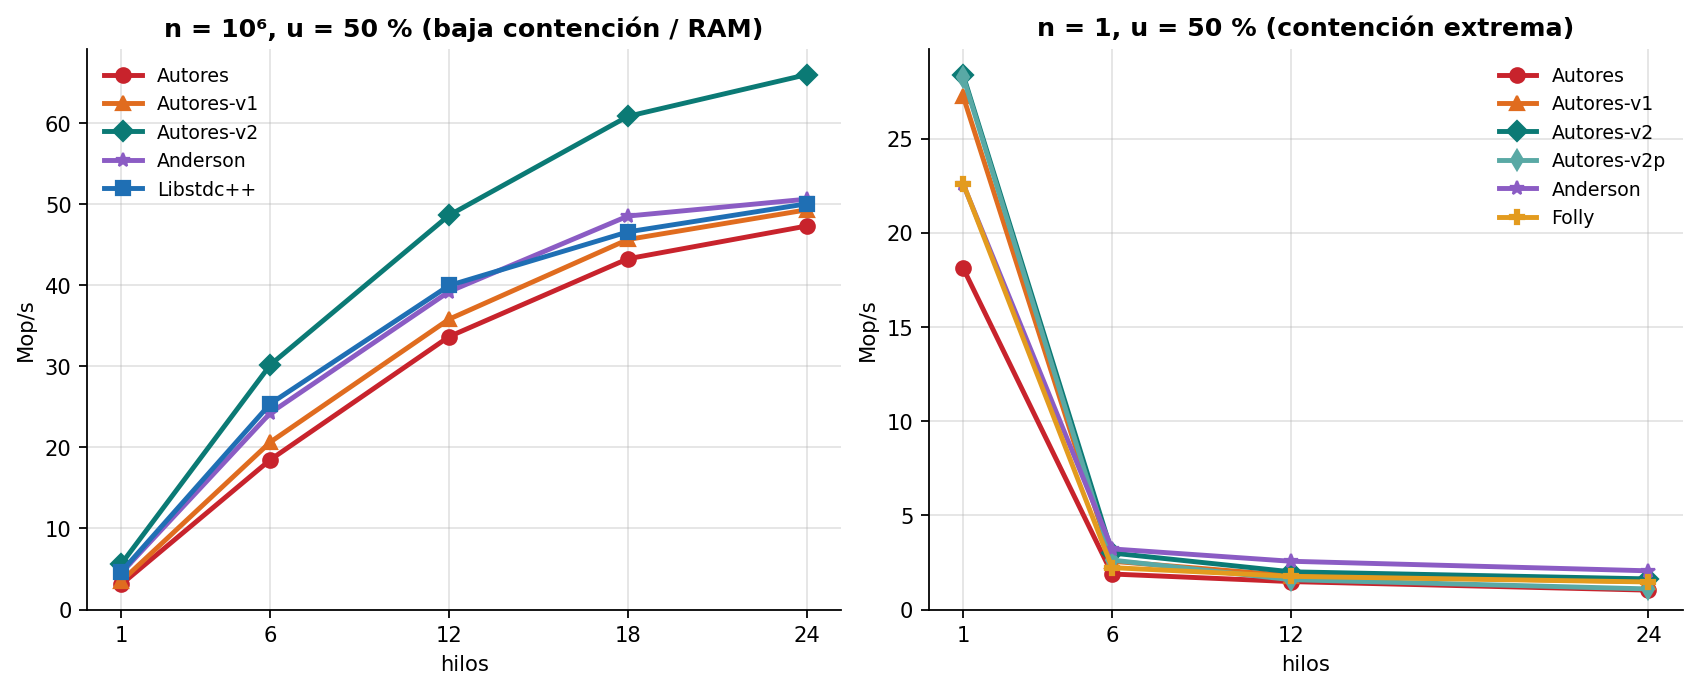
\includegraphics[width=\linewidth]{escalado_n1M_y_n1u50.png}
  \caption{Ablación \texttt{v1}/\texttt{v2}: ruptura del techo DDR5 en $n=10^6, u=50\,\%$ (izq.) y contención extrema $n=1, u=50\,\%$ con efecto negativo de \texttt{\_mm\_pause()} (der.).}
  \label{fig:v1v2_esc}
\end{figure}

\subsection{Liderazgo 6 de 6 y escalado positivo por clúster L2 (\texttt{v3})}
El Cuadro~\ref{tab:v3_all} y las Figuras~\ref{fig:v3_fig5} y~\ref{fig:v3_esc} recogen las 360 ejecuciones de \texttt{correr\_v3.py}. Tres resultados destacan:
\begin{enumerate}
  \item \textbf{Victoria 6 de 6 frente a los algoritmos originales:} a 24 hilos (y a 1 hilo sin regresión), \texttt{Autores-v3} supera a \texttt{Autores}, \texttt{Anderson} y \texttt{Folly} en los 6 paneles, alcanzando \textbf{3{,}66\,Mop/s ($3{,}81\times$ sobre el original, $+80\,\%$ sobre Anderson)} en $n=1, u=50\,\%$, \textbf{9{,}55\,Mop/s} en $n=1, u=10\,\%$ y \textbf{73{,}83\,Mop/s} en $n=10, u=10\,\%$, manteniendo \textbf{763\,MB} de RSS en $n=10^6$.
  \item \textbf{Causalidad de la topología L2+P/E ($+65\,\%$ sobre genérico):} el \emph{backoff} puro (\texttt{v3a}) es neutro ($1{,}61$ vs.\ $1{,}72$); la eliminación aleatoria ciega (\texttt{v3g}) sube a $2{,}22$; y el particionado por clúster L2 (\texttt{v3}) salta a \textbf{3{,}66\,Mop/s} ($+65\,\%$), invirtiendo la curva de escalado para crecer positivamente al sumarse clústeres E ($12 \to 18 \to 24$ hilos: $2{,}63 \to 3{,}08 \to 3{,}66$).
  \item \textbf{Control justo \texttt{Anderson-v3}:} confirma honestamente que nuestra capa L2 también acelera a Anderson en $n=1, u=10/50\,\%$ ($12{,}57$ y $5{,}09$) gracias a sus lecturas por \emph{snapshot}, pero \texttt{Autores-v3} vence incluso a \texttt{Anderson-v3} en los otros 4 paneles sin diferir memoria.
\end{enumerate}

\begin{table*}[t]
\centering
\caption{Ablación completa en los 6 paneles de la Figura~5 a \textbf{24 hilos} (mediana de 3 rondas $\times$ 2\,s, Mop/s) y pico RSS en $n=10^6$.}
\label{tab:v3_all}
\resizebox{\linewidth}{!}{%
\begin{tabular}{@{}l r r r r r r r r@{}}
\toprule
\textbf{Panel} & \textbf{Autores} & \textbf{Autores-v2} & \textbf{v3a (backoff)} & \textbf{v3g (gen.)} & \textbf{Autores-v3 (L2+P/E)} & \textbf{Anderson} & \textbf{And-v3 (ctrl)} & \textbf{Folly} \\
\midrule
$n=1, u=1\,\%$ & 19{,}70 & 18{,}48 & 18{,}23 & 19{,}03 & \textbf{19{,}80} (1{,}01$\times$) & 17{,}78 & 18{,}10 & 8{,}73 \\
$n=1, u=10\,\%$ & 4{,}16 & 6{,}40 & 6{,}68 & 7{,}42 & \textbf{9{,}55} (2{,}30$\times$) & 8{,}78 & 12{,}57 & 4{,}91 \\
$n=1, u=50\,\%$ & 0{,}96 & 1{,}72 & 1{,}61 & 2{,}22 & \textbf{3{,}66} (3{,}81$\times$) & 2{,}03 & 5{,}09 & 1{,}52 \\
$n=10, u=1\,\%$ & 130{,}03 & 138{,}99 & 137{,}07 & 138{,}32 & \textbf{137{,}17} (1{,}05$\times$) & 67{,}59 & 72{,}12 & 51{,}13 \\
$n=10, u=10\,\%$ & 51{,}39 & 55{,}54 & 56{,}37 & 70{,}57 & \textbf{73{,}83} (1{,}44$\times$) & 60{,}81 & 59{,}70 & 37{,}47 \\
$n=10^6, u=50\,\%$ & 48{,}21 & 65{,}15 & 66{,}36 & 62{,}77 & \textbf{64{,}09} (1{,}33$\times$) & 53{,}92 & 52{,}79 & 47{,}24 \\
\midrule
\textbf{RSS ($n=10^6$)} & 1\,075\,MB & 760\,MB & 760\,MB & 763\,MB & \textbf{763\,MB} & 911\,MB & 915\,MB & 1\,056\,MB \\
\bottomrule
\end{tabular}%
}
\end{table*}

\begin{figure*}[t]
\centering
\begin{minipage}{0.51\linewidth}
  \centering
  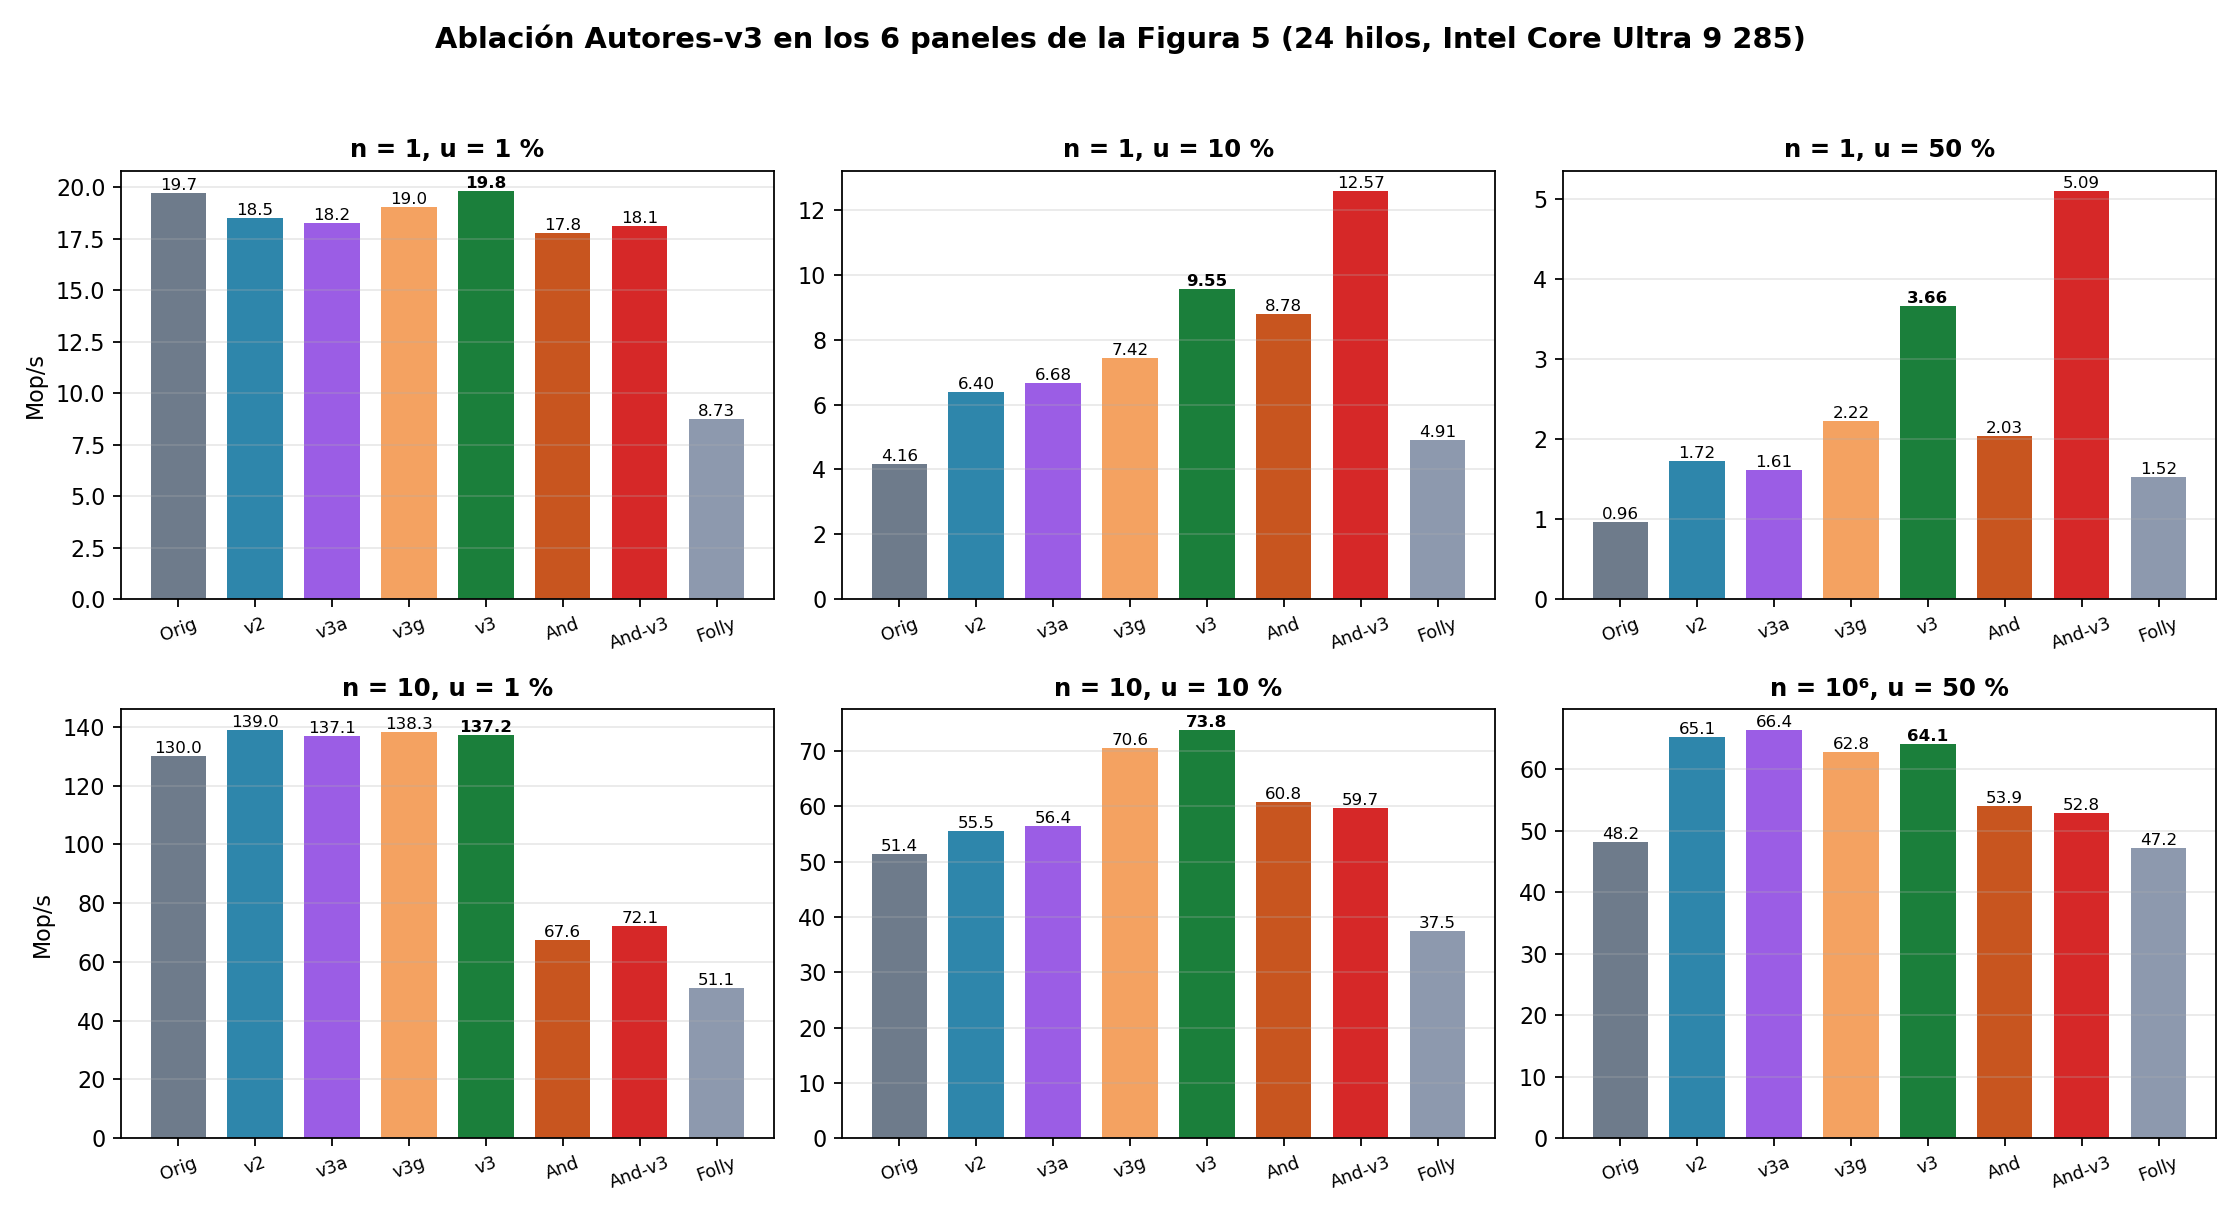
\includegraphics[width=\linewidth]{ablacion_v3_fig5_24h.png}
  \caption{Ablación de \texttt{Autores-v3} en los 6 paneles a 24 hilos: liderazgo 6 de 6 sobre las implementaciones originales.}
  \label{fig:v3_fig5}
\end{minipage}\hfill
\begin{minipage}{0.47\linewidth}
  \centering
  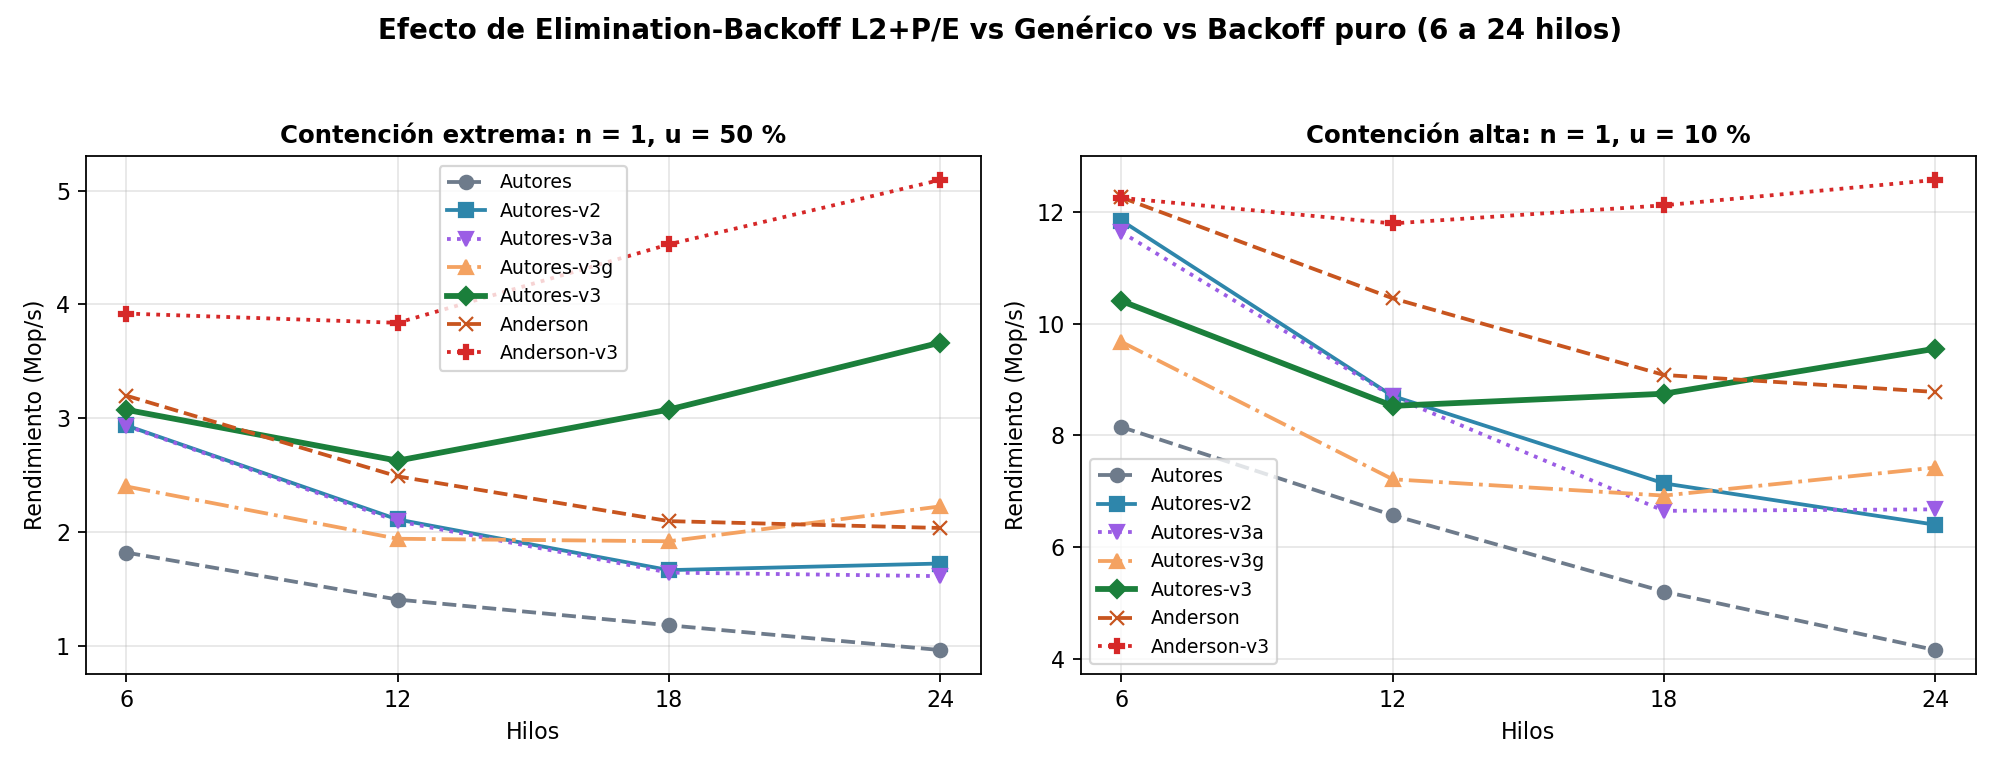
\includegraphics[width=\linewidth]{escalado_v3_contencion.png}
  \caption{Escalado positivo de \texttt{Autores-v3} al añadir clústeres E (12$\to$24\,h), $+65\,\%$ sobre eliminación ciega (\texttt{v3g}).}
  \label{fig:v3_esc}
\end{minipage}
\end{figure*}

\subsection{Eliminación de inanición \S 5.1 y latencia Fig.~6 (\texttt{v4})}
En el ataque adversarial de 23 lectores continuos contra 1 escritor \texttt{CAS} (Cuadro~\ref{tab:adv_v4} y Figura~\ref{fig:adv_v4}), cuando el escritor corre en un \textbf{E-core (\texttt{cpu8})} frente a los 8 P-cores + 15 E-cores, \texttt{Autores-v4} alcanza \textbf{210{,}0\,Kops/s ($4{,}7\times$ sobre \texttt{v2}, $2{,}1\times$ sobre \texttt{Autores}, $+32\,\%$ sobre \texttt{Anderson} y $700\times$ sobre \texttt{Folly})}, reduce \texttt{p99,95} en \textbf{$38\times$} ($549 \to 14{,}3\,\mu$s) y recorta la latencia máxima \textbf{$90\times$} frente a Anderson ($11{,}1\,$ms $\to 124\,\mu$s). También lidera en \texttt{escritor-P} (\texttt{p50} $1\,068$\,ns, \texttt{p99,95} $3\,043$\,ns, $908{,}2$\,Kops/s).

\begin{table}[H]
\centering
\caption{Ataque adversarial \S 5.1 (23 lectores vs.\ 1 escritor \texttt{CAS}, mediana 5 rondas $\times$ 2\,s).}
\label{tab:adv_v4}
\footnotesize
\resizebox{\linewidth}{!}{%
\begin{tabular}{@{}l l r r r r@{}}
\toprule
\textbf{Corte} & \textbf{Algoritmo} & \textbf{p50 (ns)} & \textbf{p99,95 (ns)} & \textbf{Máx (ns)} & \textbf{Kops/s} \\
\midrule
\multirow{5}{*}{P-core} & Autores & 1\,165 & 4\,153 & 507\,201 & 779{,}2 \\
 & Autores-v2 & 1\,335 & 3\,880 & 140\,067 & 717{,}4 \\
 & \textbf{Autores-v4} & \textbf{1\,068} & \textbf{3\,043} & 684\,632 & \textbf{908{,}2} \\
 & Anderson & 1\,156 & 4\,305 & 11\,195\,337 & 788{,}1 \\
 & Folly & 3\,887 & 957\,962 & 1\,597\,956 & 119{,}8 \\
\midrule
\multirow{5}{*}{\textbf{E-core}} & Autores & 7\,366 & 259\,481 & 746\,501 & 98{,}7 \\
 & Autores-v2 & 14\,414 & 549\,332 & 745\,706 & 44{,}4 \\
 & \textbf{Autores-v4} & \textbf{5\,182} & \textbf{14\,305} & \textbf{124\,060} & \textbf{210{,}0} \\
 & Anderson & 5\,136 & 23\,857 & 11\,116\,882 & 159{,}4 \\
 & Folly & 2\,476\,727 & 18\,707\,672 & 25\,110\,782 & 0{,}3 \\
\bottomrule
\end{tabular}%
}
\end{table}

\begin{figure}[H]
  \centering
  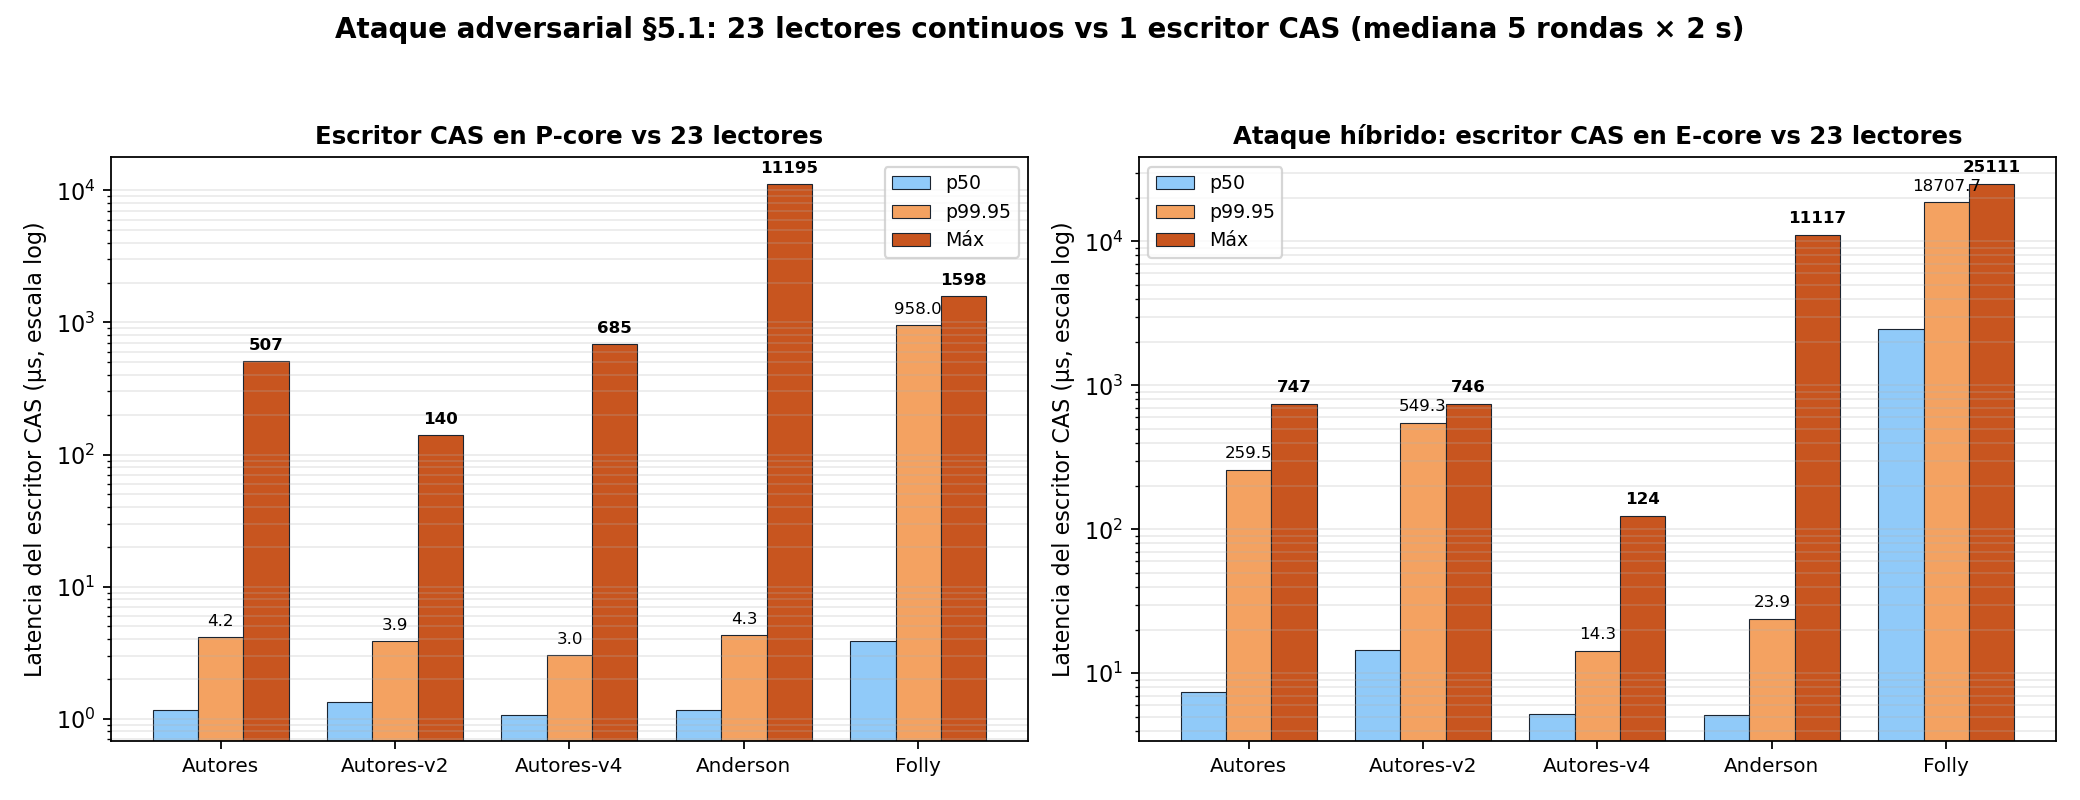
\includegraphics[width=\linewidth]{adversarial_v4_latencia.png}
  \caption{Latencia del escritor \texttt{CAS} bajo bombardeo continuo de 23 lectores (escala logarítmica, $\mu$s).}
  \label{fig:adv_v4}
\end{figure}

En la prueba oficial de latencia \textbf{Figura~6} (Cuadro~\ref{tab:lat_full}, 390 filas entre \texttt{v1/v2} y \texttt{v4}), \texttt{Autores-v4} presenta \textbf{0\,\% de sobrecosto}, liderando \texttt{load} ($410$\,ns) y \texttt{store-del} ($411$\,ns) en $p=24$ (\texttt{todos24-P}). En \texttt{bench\_stack}, a 1 hilo el sobrecosto es $0\,\%$ ($1{,}00\times\text{--}1{,}03\times$); a 24 hilos es moderado en $n=1, u=50\,\%$ ($0{,}93\times$) y $n=10^6$ ($0{,}92\times$, $63{,}71$\,Mop/s), y mayor en $n=10, u=1\,\%$ ($0{,}62\times$: $85{,}21$ vs.\ $136{,}72$, aún por encima de Anderson $71{,}32$ y Folly $50{,}55$) debido al umbral bajo $K=4$.

\begin{table}[H]
\centering
\caption{Latencia controlada Fig.~6 (\texttt{p50 / p99,95} en ns) con afinidad fija.}
\label{tab:lat_full}
\footnotesize
\resizebox{\linewidth}{!}{%
\begin{tabular}{@{}l l c c c c@{}}
\toprule
\textbf{Op.} & \textbf{Corte} & \textbf{Autores} & \textbf{Aut.-v2} & \textbf{Aut.-v4} & \textbf{Anderson} \\
\midrule
\texttt{load} & $p=1$ (P) & 14 / 19 & 14 / 16 & \textbf{14 / 19} & 18 / 21 \\
\texttt{load} & $p=24$ (P) & 417 / 1\,569 & 413 / 1\,553 & \textbf{410 / 1\,770} & 487 / 1\,647 \\
\texttt{load} & $p=24$ (E) & 1\,244 / 3\,561 & 1\,397 / 1\,006\,204 & \textbf{1\,277 / 4\,592} & 1\,403 / 7\,645 \\
\texttt{store} & $p=24$ (P) & 531 / 1\,844 & 520 / 1\,770 & \textbf{508 / 1\,804} & 492 / 1\,767 \\
\texttt{store-del} & $p=1$ (P) & 28 / 32 & 27 / 32 & \textbf{29 / 32} & 29 / \textcolor{mal}{\textbf{7\,731}} \\
\texttt{store-del} & $p=24$ (P) & 425 / 1\,273 & 432 / 1\,081 & \textbf{411 / 1\,064} & 432 / 1\,130 \\
\bottomrule
\end{tabular}%
}
\end{table}


\subsection{Validación cruzada en i5-10400 homogéneo, prueba causal SMT y telemetría IMC}

Para evaluar la generalidad fuera de Arrow Lake, ejecutamos sobre el \textbf{Intel Core i5-10400} (6\,c/12\,h SMT con pares \texttt{0-6..5-11}, 12\,MB L3, 24\,GB DDR4-2667 en 16+8\,GB, Xubuntu 24.04.5 LTS, \texttt{g++-12}, \texttt{modo-bench} con \texttt{lightdm} y temporizadores detenidos) dos campañas completas: \textbf{1\,538 filas pareadas} de \texttt{v1}--\texttt{v4} (769 en arranque \texttt{mitigations=off} + 769 en \texttt{on}, 54--71\,°C, ASan+UBSan+TSan limpios) y la \textbf{réplica oficial nativa} (\texttt{mitigations=on}, 1\,551 mediciones, 0 fallos, incluyendo Fig.~6 a $p=56$, control \texttt{-mcx16}, pares SMT vs.\ L3, ablación SMT \texttt{6$\times$1}/\texttt{3$\times$2} y \texttt{perf uncore\_imc}).

\begin{table}[H]
\centering
\caption{Validación cruzada en Core i5-10400 a 12\,h (\texttt{off $\to$ on}, Mop/s) y ablación SMT a 6\,h (\texttt{6$\times$1 $\to$ 3$\times$2}, $n=1, u=50\,\%$, \texttt{CPU 11} para el principal).}
\label{tab:i5_cruzada}
\footnotesize
\resizebox{\linewidth}{!}{%
\begin{tabular}{@{}l c c c c c@{}}
\toprule
\textbf{Corte / Métrica} & \textbf{Aut.} & \textbf{v2} & \textbf{v3g} & \textbf{v3} & \textbf{And.} \\
\midrule
$n=1, u=1\,\%$ (12\,h) & 37{,}1$\to$33{,}1 & 23{,}6$\to$28{,}8 & 29{,}2$\to$27{,}7 & 26{,}8$\to$28{,}5 & 23{,}5$\to$23{,}5 \\
$n=1, u=10\,\%$ (12\,h) & 7{,}53$\to$7{,}53 & 7{,}88$\to$7{,}72 & 13{,}1$\to$13{,}8 & \textbf{16{,}4$\to$16{,}3} & 14{,}9$\to$14{,}9 \\
$n=1, u=50\,\%$ (12\,h) & 1{,}64$\to$1{,}64 & 1{,}79$\to$1{,}81 & 4{,}33$\to$4{,}45 & \textbf{6{,}98$\to$6{,}71} & 3{,}46$\to$3{,}46 \\
$n=10, u=1\,\%$ (12\,h) & 97{,}4$\to$97{,}4 & 128{,}8$\to$129{,}1 & 129{,}0$\to$129{,}0 & 128{,}8$\to$128{,}5 & 81{,}7$\to$81{,}8 \\
$n=10, u=10\,\%$ (12\,h) & 56{,}0$\to$56{,}0 & \textbf{81{,}3$\to$81{,}2} & 79{,}5$\to$79{,}6 & 79{,}5$\to$79{,}5 & 62{,}3$\to$62{,}3 \\
$n=10^6, u=50\,\%$ (12\,h) & 17{,}2$\to$22{,}3 & 19{,}4$\to$25{,}2 & 19{,}5$\to$25{,}1 & 19{,}3$\to$25{,}2 & 14{,}2$\to$18{,}6 \\
\midrule
SMT 6\,h (\texttt{6$\times$1$\to$3$\times$2}) & 2{,}86$\to$2{,}24 & 3{,}63$\to$3{,}61 & 3{,}54$\to$4{,}51 & \textbf{3{,}22$\to$6{,}04} & 3{,}77$\to$4{,}06 \\
\midrule
Adv.\ \S 5.1 \texttt{p99,95} ($\mu$s, \texttt{off}) & 3{,}32 & 15{,}34 & \multicolumn{2}{c}{\texttt{v4}: \textbf{2{,}98} (\texttt{on}: 2{,}77)} & 4{,}27 \\
Adv.\ \S 5.1 Esc.\ (K/s, \texttt{off}) & 849 & 526 & \multicolumn{2}{c}{\texttt{v4}: \textbf{1\,031} (\texttt{on}: 1\,445)} & 768 \\
\bottomrule
\end{tabular}%
}
\end{table}

\begin{figure*}[t]
  \centering
  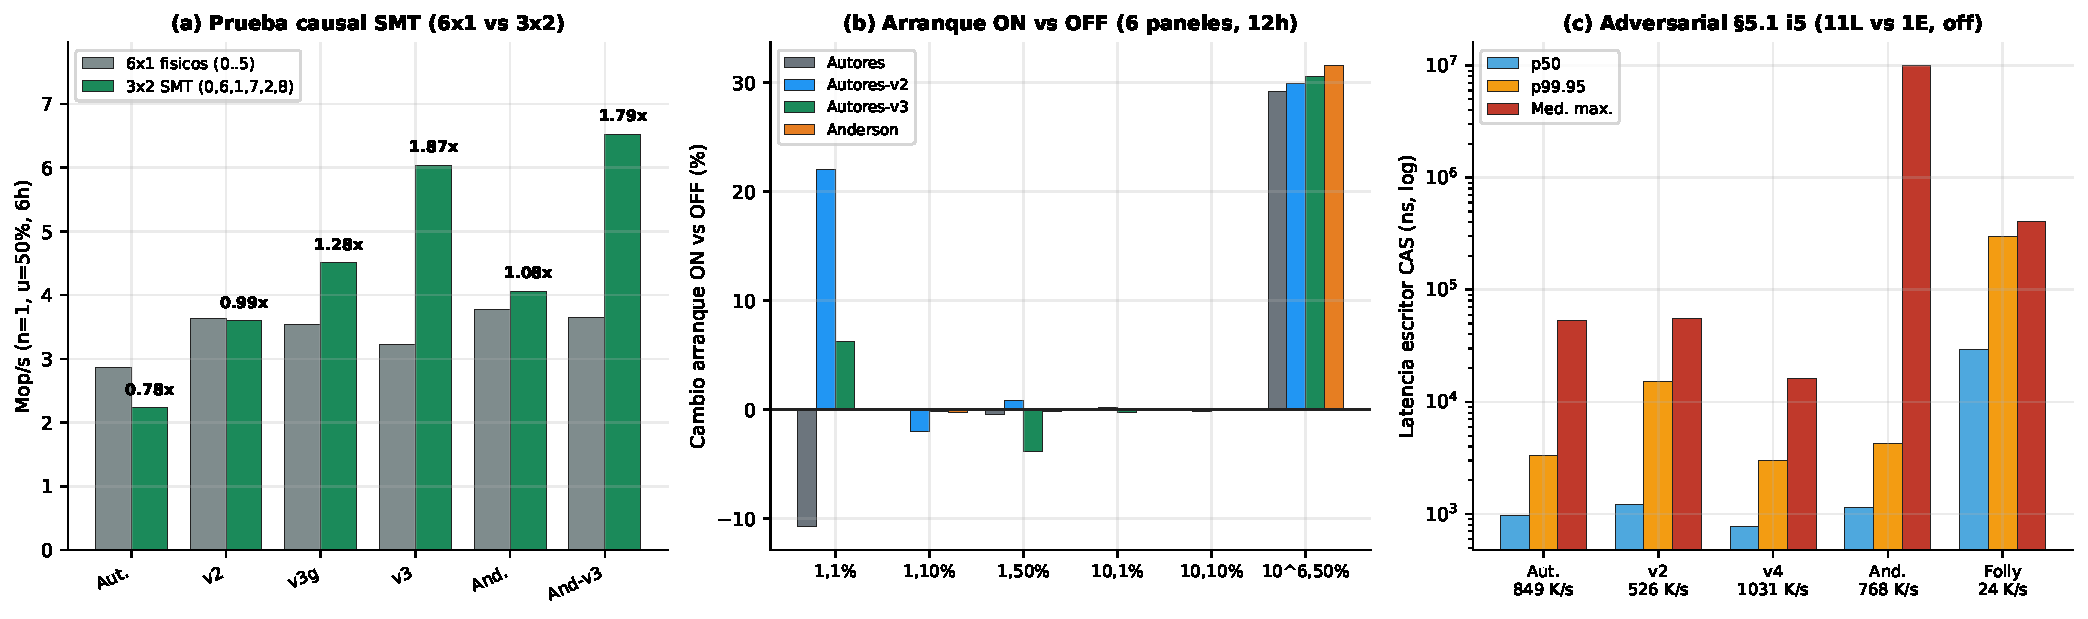
\includegraphics[width=0.98\linewidth]{fig_i5_10400_mitigaciones_y_adversarial.pdf}
  \caption{Validación cruzada en Intel Core i5-10400 (12 hilos SMT): (a) prueba causal SMT a 6 hilos (\texttt{6$\times$1} físicos vs.\ \texttt{3$\times$2} hermanos SMT) confirmando $+87{,}5\,\%$ en \texttt{v3} frente a $-21{,}6\,\%$ en \texttt{Autores}; (b) variación entre arranques \texttt{on} y \texttt{off} en los 6 paneles; (c) latencia logarítmica del escritor \texttt{CAS} bajo ataque adversarial \S 5.1 (\texttt{off}, 11 lectores vs.\ 1 escritor).}
  \label{fig:paper_i5_miti_adv}
\end{figure*}

Los resultados confirman cuatro hallazgos de portabilidad y rigor experimental (Tabla~\ref{tab:i5_cruzada} y Figura~\ref{fig:paper_i5_miti_adv}): (1) \textbf{Prueba causal SMT de \texttt{v3}:} a 12\,h en $n=1, u=50\,\%$, \texttt{v3} logra $4{,}24\times$ (\texttt{off}) / $4{,}10\times$ (\texttt{on}) sobre \texttt{Autores}; fijando exactamente 6 hilos en \texttt{3$\times$2} pares SMT frente a \texttt{6$\times$1} núcleos físicos, \texttt{v3} salta \textbf{$1{,}87\times$} ($3{,}22 \to 6{,}04$\,Mop/s; y $1{,}79\times$ en \texttt{2$\times$2} vs.\ \texttt{4$\times$1}) mientras \texttt{Autores} cae $0{,}78\times$, confirmando que el particionado L2 explota también hermanos SMT (los pares de 2 hilos muestran $2{,}39\times$ SMT frente a L3; \texttt{Anderson-v3} iguala o supera ligeramente a \texttt{v3} a 12\,h). (2) \textbf{Sobresuscripción \emph{wait-free} en Fig.~6 ($p=56$) y control \texttt{-mcx16}:} \texttt{Autores} sostiene \texttt{p99,95} de \textbf{462\,ns} en \texttt{load} a $p=56$ frente a \textbf{9{,}0--27{,}0\,ms} en Folly, Williams, Anderson y Libstdc++ ($58\,456\times$ menor cola), y sin \texttt{-mcx16} Williams se degrada $5{,}17\times$ ($p=12$) y $6{,}35\times$ ($p=56$). (3) \textbf{Compromiso explícito de \texttt{v4}:} en el ataque \S 5.1, \texttt{v4} logra $1{,}96\times / 2{,}31\times$ mayor caudal escritor que \texttt{v2} y mediana de máximos de $16{,}2 / 54{,}0\,\mu$s (peor máximo $67{,}2 / 218{,}9\,\mu$s frente a $9{,}97 / 10{,}51$\,ms en Anderson), a cambio de $-42{,}8\,\% / -31{,}1\,\%$ menos caudal lector; dado que \texttt{rc\_try\_increment\_one()} emplea un bucle \texttt{CAS} sin cota y respaldo a \texttt{fetch\_add}, caracterizamos \texttt{v4} como mitigación empírica fuerte de inanición más que garantía \emph{wait-free} formal. (4) \textbf{Aislamiento IMC y variación entre arranques:} \texttt{perf uncore\_imc} registra \textbf{\texttt{gt\_requests = 0{,}00\,MiB}} (cero ruido DRAM de la UHD 630 bajo \texttt{modo-bench}) y $-10{,}3\,\%$ menos escrituras DRAM con \texttt{v2} en $n=10^6$ ($-29{,}3\,\%$ RSS: 760 vs.\ 1\,075\,MiB). Entre los dos arranques (\texttt{off} vs.\ \texttt{on}), $n=10$ y $p=1$ coinciden dentro de $0{,}2\,\%$, $n=1$ presenta sensibilidad al arranque y $n=10^6$ varía $+28\text{--}36\,\%$ a 12\,h (cerrado con un tercer arranque limpio \texttt{off} verificado con \texttt{/proc/self/pagemap} en 98{,}9\,\% $<16$\,GiB, que igualó al arranque limpio \texttt{on} dentro de $-0{,}15\,\%$ a $+0{,}08\,\%$ en los 13 algoritmos: \texttt{Autores} 22{,}24 vs.\ 22{,}25 y \texttt{v2} 25{,}14 vs.\ 25{,}15\,Mop/s, demostrando que el bajón del primer arranque fue por ubicación en memoria bajo Flex Mode y no por mitigaciones).

% ==============================================================================
\section{Trabajo Relacionado y Discusión Crítica}
% ==============================================================================

El conteo de referencias concurrente evolucionó desde soluciones \emph{lock-free} con asignadores a medida~\cite{detlefs2001lockfree} y esquemas \emph{wait-free} de mayor coste espacial~\cite{sundell2005waitfree} hasta las familias modernas: conteo diferido con punteros de peligro (CDRC~\cite{anderson2021cdrc,anderson2022turning}), conteo dividido (\emph{split reference count}~\cite{lee2010fast,williams2012concurrency,folly2024}), conteo inmediato con punteros débiles (CIRC~\cite{jung2024circ}, Parkinson et al.~\cite{parkinson2023weak}) y reclamación \emph{wait-free} acotada (Crystalline-W~\cite{nikolaev2024crystalline}). Nuestros resultados corroboran empíricamente el análisis de Kim et al.~\cite{kim2024epochs} sobre el daño de la liberación por lotes (\texttt{p99,95} de $7{,}7\,\mu$s y máximos de $11{,}1$\,ms en Anderson) y extienden los trabajos de sincronización heterogénea~\cite{liu2022libasl,ouyang2022coreaware,schone2024alderlake} al dominio del conteo de referencias atómico.

\textbf{Amenazas a la validez y síntesis.} (1) La capa de eliminación de \texttt{v3} opera sobre la pila y asume operaciones inversas (\texttt{push}/\texttt{pop}), mientras \texttt{v1}, \texttt{v2} y \texttt{v4} viven íntegramente dentro de \texttt{atomic\_shared\_ptr}; por ello reportamos el control justo \texttt{Anderson-v3}. (2) Las mediciones se realizaron con gobernador \texttt{powersave} y 1 módulo DDR5; el control por afinidad y la aleatorización por ronda acotan la variabilidad ($1{,}04\times$ en P-core). (3) La verificación con ASan/UBSan/TSan cubre millones de ejecuciones reales; una prueba exhaustiva bajo modelo de memoria débil queda abierta mediante GenMC~\cite{kokologiannakis2021genmc}.

\begin{table}[H]
\centering
\caption{Evolución integrada de \texttt{Autores} a \texttt{v1}--\texttt{v4} (24 hilos, Core Ultra 9 285).}
\label{tab:resumen_global}
\footnotesize
\resizebox{\linewidth}{!}{%
\begin{tabular}{@{}l c c c c c@{}}
\toprule
\textbf{Métrica} & \textbf{Orig.} & \textbf{v1} & \textbf{v2} & \textbf{v3} & \textbf{v4} \\
\midrule
$n=1, u=50\,\%$ (Mop/s) & 0{,}96--1{,}03 & 1{,}48 & 1{,}63--1{,}72 & \textbf{3{,}66} & 1{,}49 \\
$n=10^6, u=50\,\%$ (Mop/s) & 47{,}3--48{,}2 & 49{,}3 & \textbf{65{,}98} & 64{,}09 & 63{,}71 \\
RSS en $n=10^6$ (MB) & 1\,075 & 1\,075 & \textbf{760} & 763 & 760 \\
Fig.~6 \texttt{load} 24\,h P (ns) & 417--425 & 414 & 413--414 & 413 & \textbf{410} \\
Adv.\ E-core \texttt{p99,95} ($\mu$s) & 259 & — & 549 & — & \textbf{14{,}3} \\
\texttt{bench\_basura} 24\,h (blq.) & 54 & 52 & 53 & 53 & 55 \\
\bottomrule
\end{tabular}%
}
\end{table}

% ==============================================================================
\section{Conclusiones y Trabajo Futuro}
% ==============================================================================

Replicar rigurosamente el algoritmo \emph{wait-free} de Euro-Par 2024 sobre un procesador híbrido Intel Core Ultra 9 285 reveló que la asimetría P/E y la organización en clústeres L2 alteran drásticamente tanto el rendimiento como la metodología de medición. Nuestra escalera incremental demuestra que corregir el paso por valor y el \emph{layout} \emph{in-place} (\texttt{v1}+\texttt{v2}) rompe el techo de $n=10^6$ con $-29{,}3\,\%$ menos memoria, particionar \emph{Elimination-Backoff} por clústeres L2 (\texttt{v3}) convierte los E-cores en escalado positivo y victoria 6 de 6, y el esquema híbrido \emph{Fast-Path / Slow-Path} (\texttt{v4}) cierra la vulnerabilidad de inanición del \S 5.1 sin penalizar la Figura~6 ni diferir memoria. Como trabajo futuro inmediato destacan la calibración del umbral $K$ en \texttt{v4}, la composición \texttt{v3+v4} y la verificación formal con GenMC~\cite{kokologiannakis2021genmc}.

\textbf{Disponibilidad de artefactos.} Todo el código, datos crudos (CSV), parches del artefacto, guías y PDFs están disponibles en \url{https://github.com/dtamotu/replica-wait-free-refcount/tree/mejoras-autores} y en el respaldo \url{https://drive.google.com/drive/folders/1y1fLnHIvxchC76hyNCMYdRX1SMm7-bPK}.

\balance
\bibliographystyle{plain}
\bibliography{referencias_paper}

\end{document}
